%%%%%%%%%%%%%%%%%%%%%%%%%%%%%%%%%%%%%%%%%
% Short Sectioned Assignment
% LaTeX Template
% Version 1.0 (5/5/12)
%
% This template has been downloaded from:
% http://www.LaTeXTemplates.com
%
% Original author:
% Frits Wenneker (http://www.howtotex.com)
%
% License:
% CC BY-NC-SA 3.0 (http://creativecommons.org/licenses/by-nc-sa/3.0/)

%%%%%%%%%%%%%%%%%%%%%%%%%%%%%%%%%%%%%%%%%

%----------------------------------------------------------------------------------------
% PACKAGES AND OTHER DOCUMENT CONFIGURATIONS
%----------------------------------------------------------------------------------------

\documentclass[paper=a4, fontsize=11pt]{scrartcl} % A4 paper and 11pt font size
%\usepackage[icelandic]{babel}
\usepackage[none]{hyphenat}
\usepackage[usenames,dvipsnames]{color} %litir
\usepackage[colorlinks]{hyperref}
\usepackage{subfig}
\usepackage[T1]{fontenc} % Use 8-bit encoding that has 256 glyphs
\usepackage{fourier} % Use the Adobe Utopia font for the document - comment this line to return to the LaTeX default
\usepackage{mathtools}
\usepackage{amsfonts}
\usepackage{amsthm}
\usepackage[utf8x]{inputenc}
%\usepackage[utf8]{inputenc} %Íslenskir stafir
\usepackage{enumerate} %list
\usepackage{graphicx}
\usepackage{color}
\usepackage{fullpage}
\usepackage[nottoc,numbib]{tocbibind}
\usepackage{lipsum} % Used for inserting dummy 'Lorem ipsum' text into the template
\usepackage{listings} %Fyrir Kóðann
\lstset{  
  literate=
  {á}{{\'{a}}}1
  {Á}{{\'{A}}}1
  {ð}{{\dh}}1
  {Ð}{{\DH}}1
  {é}{{\'{e}}}1
  {É}{{\'{E}}}1
  {í}{{\'{i}}}1
  {Í}{{\'{I}}}1
  {ó}{{\'{o}}}1
  {Ó}{{\'{O}}}1
  {ý}{{\'{y}}}1
  {Ý}{{\'{Y}}}1
  {ú}{{\'{u}}}1
  {Ú}{{\'{U}}}1
  {þ}{{\TH}}1
  {Þ}{{\th}}1
  {æ}{{\ae}}1
  {Æ}{{\AE}}1
  {ö}{{\"{o}}}1
  {Ö}{{\"{O}}}1,
  stringstyle=\ttfamily\color{BurntOrange},
  showstringspaces=false,
  basicstyle=\small,
  numberstyle=\footnotesize,
  numbers=left,
  stepnumber=1,
  numbersep=10pt,
  tabsize=2,
  caption=\lstname,
  breakatwhitespace=false,
  aboveskip={1.5\baselineskip},
  language=Java,
  keywordstyle=\bfseries\ttfamily\color{ProcessBlue},
  identifierstyle=\ttfamily,
  commentstyle=\color{OliveGreen},
  prebreak = \raisebox{0ex}[0ex][0ex]{\ensuremath{\hookleftarrow}},
  breakatwhitespace=false,
  aboveskip={1.5\baselineskip},
  frame=single,
}
\usepackage{sectsty} % Allows customizing section commands
\allsectionsfont{\normalfont\scshape} % Make all sections centered, the default font and small caps
\setcounter{tocdepth}{2}
\usepackage{fancyhdr} % Custom headers and footers
\pagestyle{fancyplain} % Makes all pages in the document conform to the custom headers and footers
\fancyhead{} % No page header - if you want one, create it in the same way as the footers below
\fancyfoot[L]{} % Empty left footer
\fancyfoot[C]{} % Empty center footer
\fancyfoot[R]{\thepage} % Page numbering for right footer
\renewcommand{\headrulewidth}{0pt} % Remove header underlines
\renewcommand{\footrulewidth}{0pt} % Remove footer underlines
\setlength{\headheight}{13.6pt} % Customize the height of the header
\bibliographystyle{abbrv}

\numberwithin{equation}{section} % Number equations within sections (i.e. 1.1, 1.2, 2.1, 2.2 instead of 1, 2, 3, 4)
\numberwithin{figure}{section} % Number figures within sections (i.e. 1.1, 1.2, 2.1, 2.2 instead of 1, 2, 3, 4)
\numberwithin{table}{section} % Number tables within sections (i.e. 1.1, 1.2, 2.1, 2.2 instead of 1, 2, 3, 4)

\setlength\parindent{1cm} % Removes all indentation from paragraphs - comment this line for an assignment with lots of text

%----------------------------------------------------------------------------------------
% TITLE SECTION
%----------------------------------------------------------------------------------------

\newcommand{\horrule}[1]{\rule{\linewidth}{#1}} % Create horizontal rule command with 1 argument of height

\title{ 
\normalfont \normalsize 

\includegraphics[width=0.25\textwidth]{logo.jpg}~\\[1cm]
\textsc{Háskóli Íslands} \\ [25pt] % Your university, school and/or department name(s)
\horrule{0.5pt} \\[0.4cm] % Thin top horizontal rule
\huge {Final Report \\ BS in Computer Science} % The assignment title
\horrule{2pt} \\[0.5cm] % Thick bottom horizontal rule
}

\author{Svavar Árni Halldórsson} % Your name
%{Dæmakennari: }
%{\normalsize }
\date{\normalsize Due 5. June 2015} % Today's date or a custom date

\begin{document}

\maketitle
\clearpage

\hypersetup {
  linkcolor = black
}
\tableofcontents
\hypersetup {
  linkcolor = ForestGreen,
  urlcolor = ForestGreen
}
\clearpage
\section{Introduction}
This report describes the preparation and execution of my final project for my B.S. in computer science. The project initiated from my interest in web development as well as a fascination with the card game Magic the Gathering. The goal of this project is to study different methods in developing websites, setting up databases and overall make a functional and user friendly site. This report describes a simple website where a user can further immerse himself in searching, browsing and studying all the cards available in the game. The system itself will use Magic the Gathering as a premise but the most important thing will be a prototype mini version of a application, with 
 \\ requirement analysis and usability studies and the study of ASP.NET MVC, using Visual Studio. The first part of this report describes the requirement analysis, followed by the preliminary design phase, ending with an overview of the production process itself. The last parts of this report contain the conclusion and references.

\section{About the System}
Magic was the first trading card game produced and it continues to thrive, with approximately twelve million players as of 2011. Magic can be played by two or more players each using a deck of 60+ printed cards or a deck of virtual cards through the Internet Based Magic: The Gathering Online. An organized tournament system and a community of professional Magic players has developed, as has a secondary market for Magic cards. Magic cards can be valuable due to their rarity and utility in gameplay (\href{http://en.wikipedia.org/wiki/Magic:_The_Gathering}{further information}).
  
This system, called Magic Builder, is meant as a reference guide for Magic players to search and browse cards, view detail information about them and build deck of cards. Magic Builder will allow a user to register an account and build decks on his own profile.

\section{Competition}
\subsection{mtg vault}
This website is an extensive library of Magic The Gathering information. The website mostly centers around viewing decks from other users and sharing your own. The card search is advanced and gives a lot of options. Overall the website works pretty well and is easy to use. The biggest flaws I noticed while researching MtgVault concern the look and feel of the site, it looks dated and unresponsive, when using the card search or clicking items the page executes a full reload and most importantly the page is not scalable and therefore only works on desktop computers.
(\href{http://www.mtgvault.com/}{mtg vault}).
\subsection{What can be simulated}
Magic builder will feature a lot of the same functions as mtgVault such as searching for cards and building decks, however my goal is to make Magic builder simple, fast and available on all screen sizes. 

\clearpage

\section{The Average User}
To better visualize how the system would be used, I felt that it was important to analyze a typical user of a system of this kind.
\subsection{Background}
The average system user will be in the age range 20 - 40, any gender and have an elementary education or more. The user will most likely have good computer experience and have minimal disabilities, although poor eyesight could be a factor.
\subsection{System Use}
The average user will use the system any day of the week, with possible spikes on the weekends and average use will probably be around once per week. There should be no training necessary and the user should have a very positive attitude towards the system.
\subsection{Environment}
\begin{itemize}
  \item Technical Environment \\
  The system will be used on desktop computers, laptops, tablets or other similar devices.
  \item Real Environment \\
  The system will be used in any environment, i.e. at home, work, in school, or other institutions and places.
\end{itemize}
\subsection{Main Goals}
The average user will use the system to make an account, search and browse cards and make decks. Possibly connect with other players and share ideas.

\clearpage

\section{Requirements}
The following is a list of functionalities that the user can do within the system. They are ordered by priority A, B or C. Requirements with priority A are essential, B are features that are important but not critical and C are nice to have features. The numbers in the user stories column refer to user stories with the corresponding numbers.
\subsection{Functional Requirements}
\begin{center}
  \makebox[\textwidth]{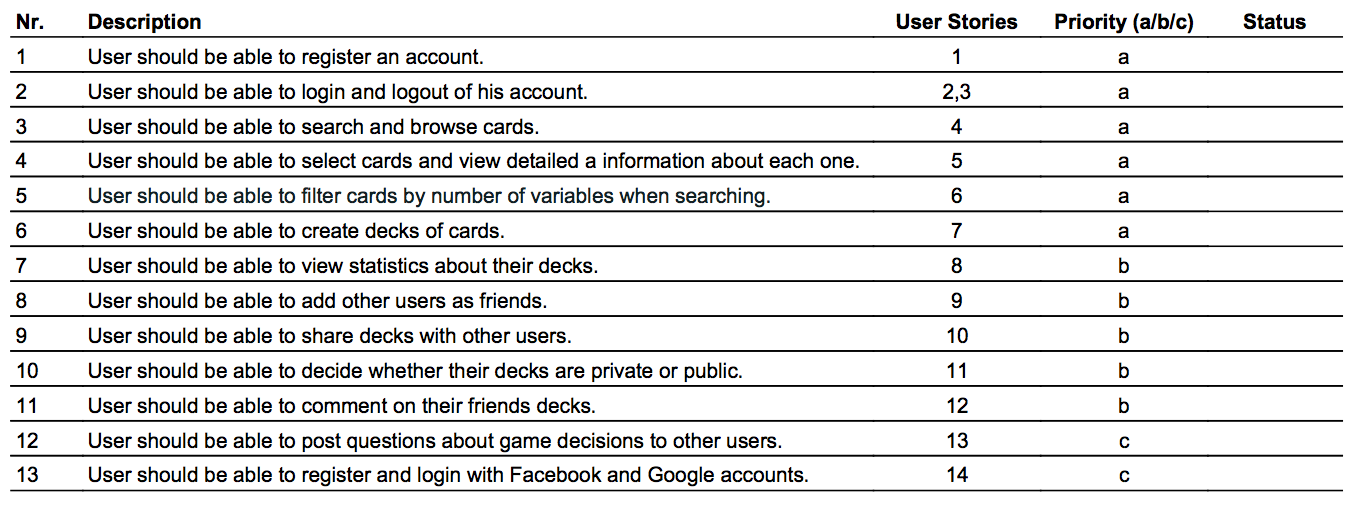
\includegraphics[width=1\textwidth]{RequirementList.png}}
\end{center}
\subsection{Non-functional Requirements}
\begin{center}
  \makebox[\textwidth]{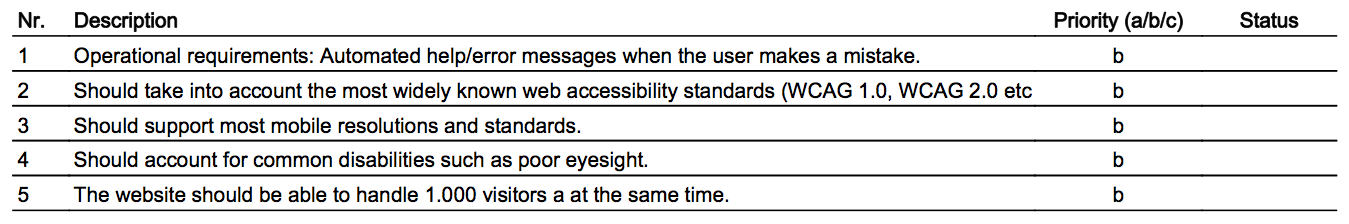
\includegraphics[width=1\textwidth]{non-functional.png}}
\end{center}

\clearpage

\section{User Stories}
The user stories describe the requirements in an everyday language. They also suggest a reason for wanting to be able to complete the tasks. They are meant to be simple and easy to understand and should make a good checklist when implementing the system. The user stories are ordered by priority, with the red boxes containing the highest priority stories, the yellow the intermediate ones and the green the lowest priority. Although the yellow and green user stories might not be implemented they are nevertheless included in case the organization of the project, or the priority of the user stories, changes in any way.
\begin{center}
  \makebox[\textwidth]{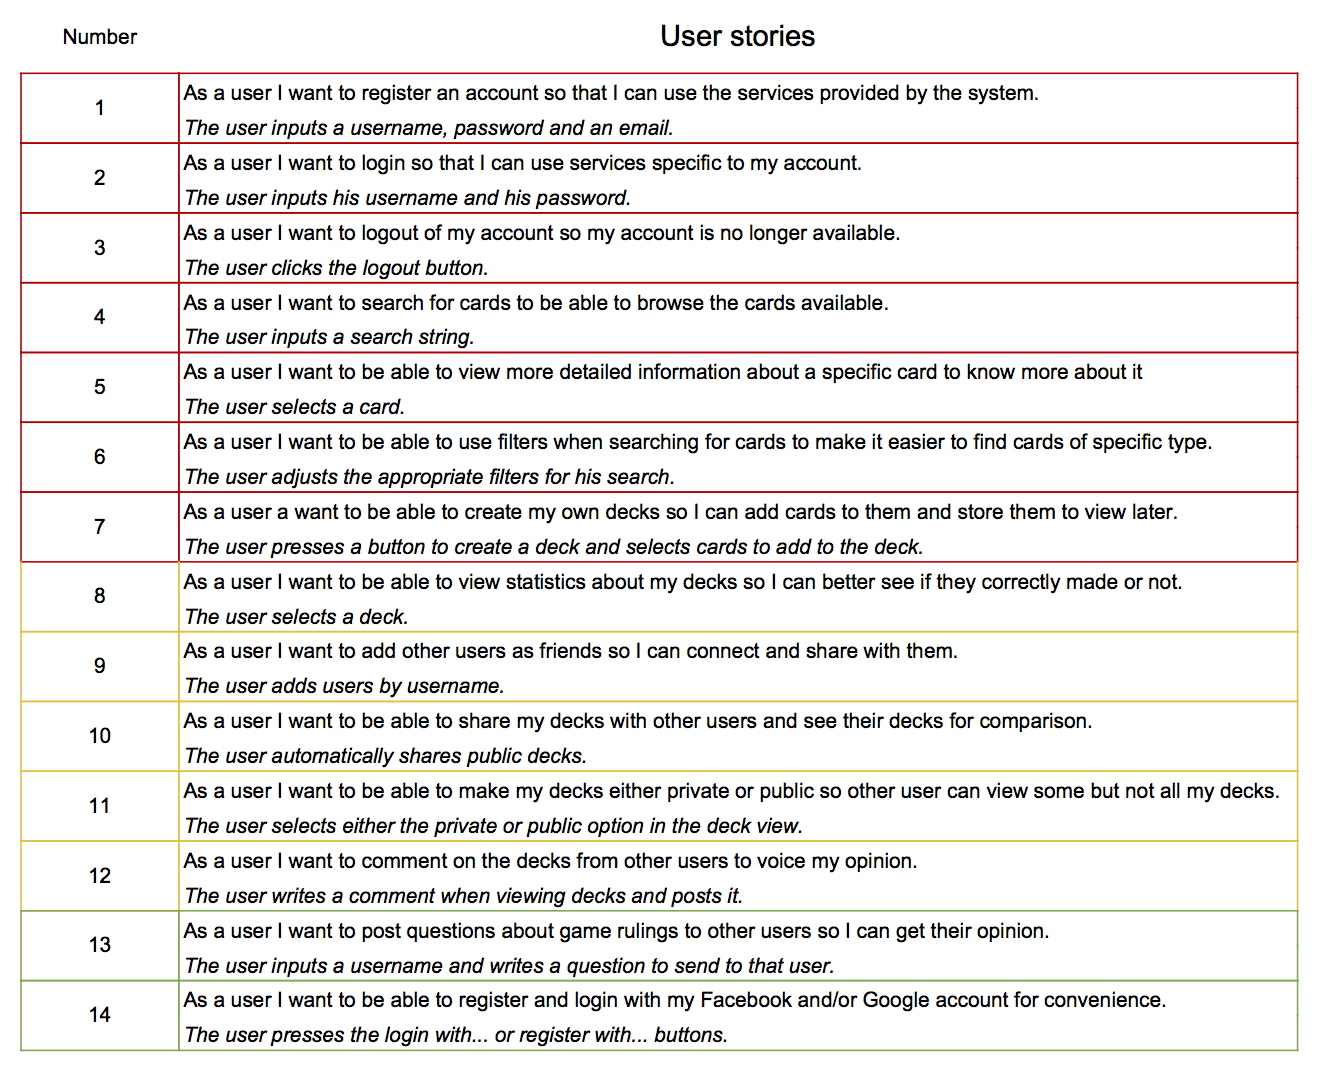
\includegraphics[width=1\textwidth]{UserStories.png}}
\end{center}

\clearpage

\section{Usability Goals}
I decided to set a few target goals for new users, if more than 80\% of them are able to perform the tasks with the given constraints then the system’s usability is satisfactory, but of course experienced users should easily be able to outperform the constraints.
\begin{itemize}
  \item The user should be able to register an account in under 2 minutes.
  \item The user should be able to login in less than 20 seconds.
  \item The user should be able to search for a card in less than a minute.
  \item The user should be able to create a deck in less than a minute.
  \item The user should be able to log out in less than 20 seconds.
  \item The user should be able to get to the homepage in one click from any page.
\end{itemize}

\section{Prototypes}
For the first draft layout of the website I made a few wireframes that give a good overview of the website. I also made some graphic design prototypes for reference but they do not necessarily portray the final look of the website since functionality will always be the highest priority.
\subsection{Wireframes}
The first wireframe describes the front page of the website. It has the same layout as all other pages on the site but if the user is not logged in he will be prompted with the register option in the top right corner of the page but the logout option otherwise.
\begin{center}
  \makebox[\textwidth]{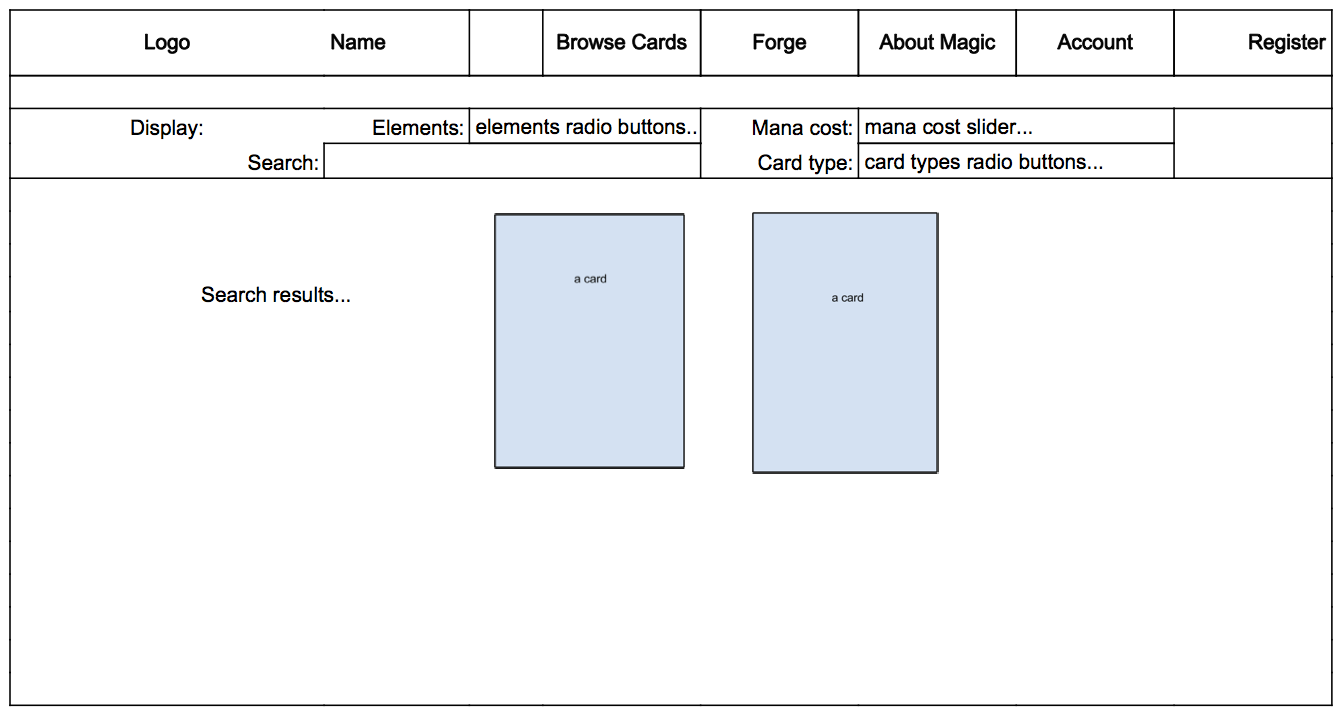
\includegraphics[width=1\textwidth]{WireframeFrontPage.png}}
\end{center}
\clearpage

The login page will also have the same layout as the other pages but display a login form where the user can insert his login information or press register if the user doesn’t have an account. The register page is the same as the login page except it displays a register form.
\begin{center}
  \makebox[\textwidth]{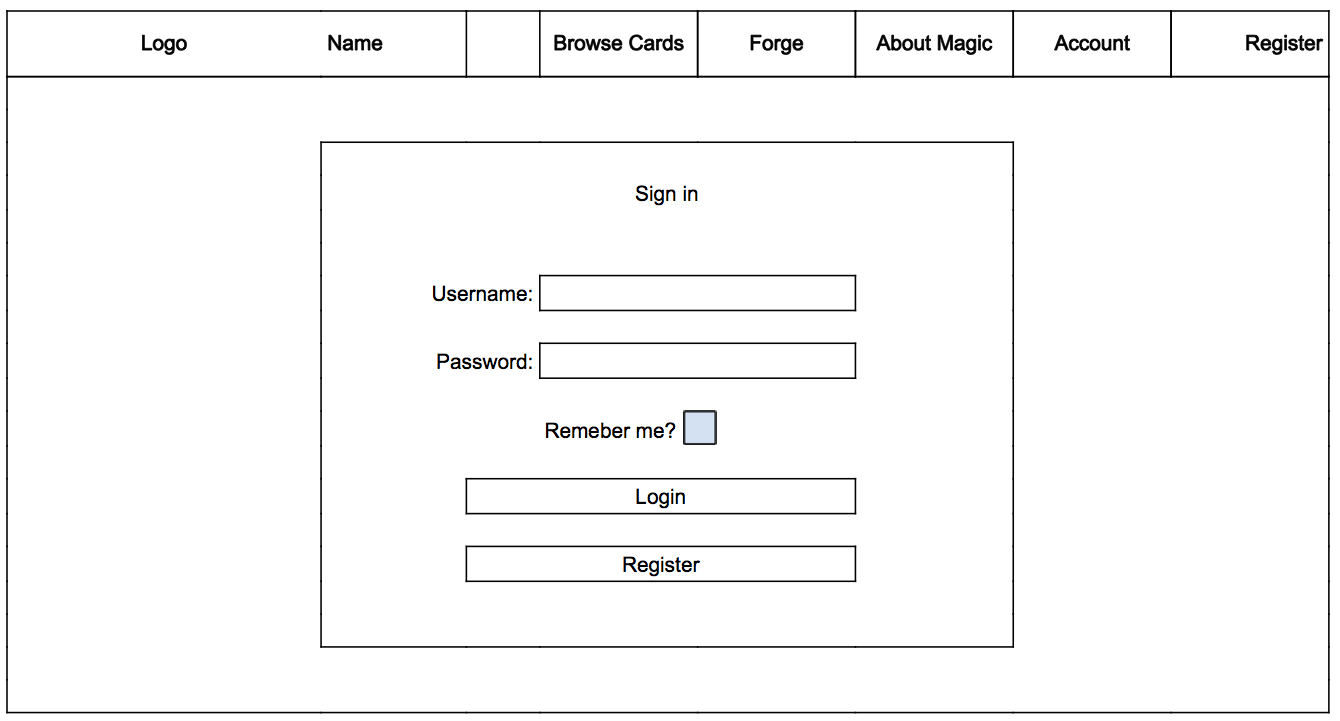
\includegraphics[width=1.1\textwidth]{WireframeSignIn.png}}
\end{center}
The forge is only available for logged in user. It has the same layout as other pages but displays the logout option in the top right corner. It gives the user the options to view their favorite cards, create new decks or navigate between already made decks and has the same search as the front page where the user can search for cards and add them to their decks. The current deck is then displayed below.
\begin{center}
  \makebox[\textwidth]{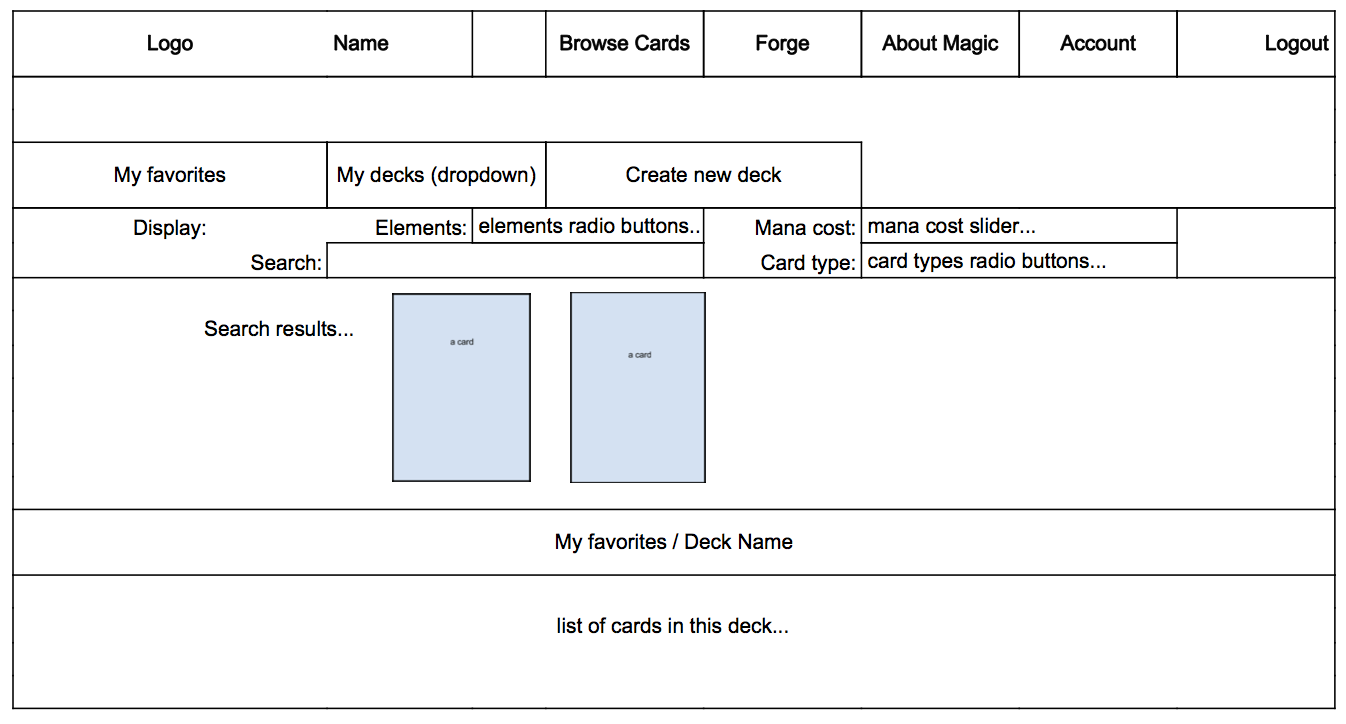
\includegraphics[width=1.1\textwidth]{forge.png}}
\end{center}
The about magic page will have the same layout as the others with either logout or register in the top right corner, depending on whether the user is logged in or not. The main area will then display a tab bar that a user can use to exchange the information displayed.
\begin{center}
  \makebox[\textwidth]{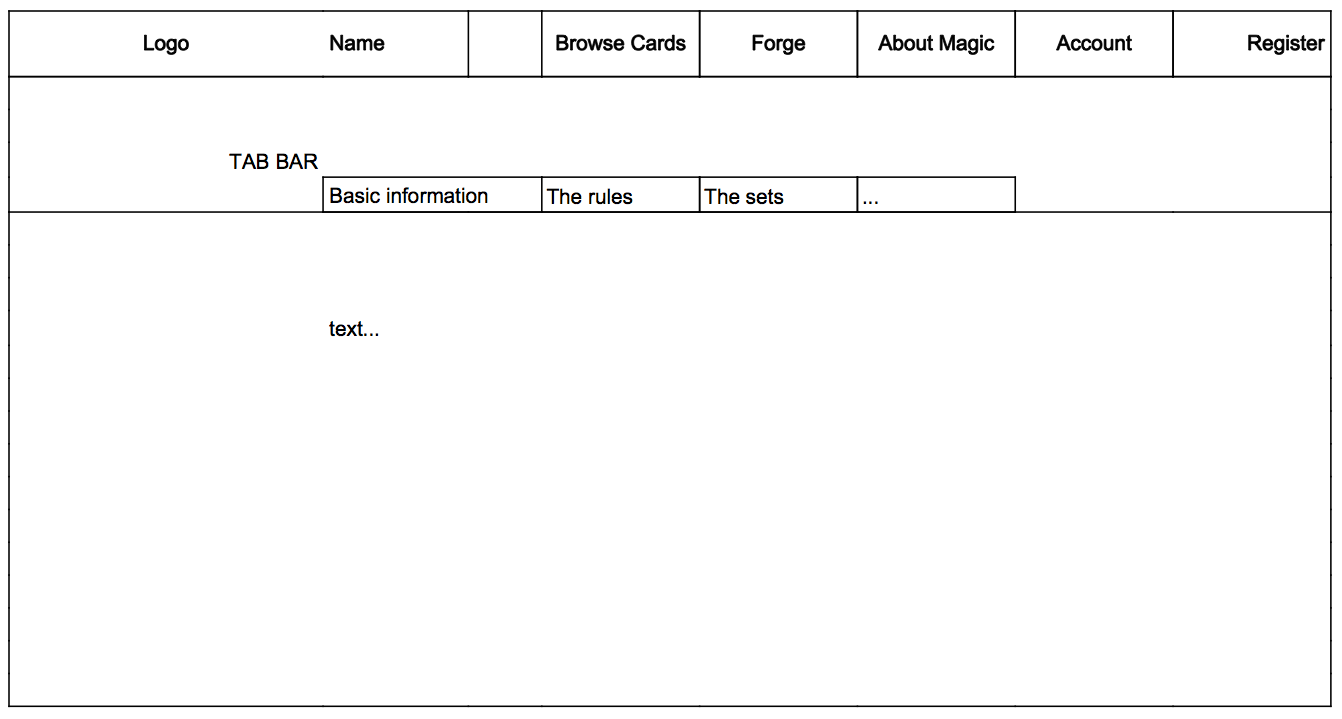
\includegraphics[width=1.1\textwidth]{aboutMagic.png}}
\end{center}

\subsection{Graphic Design}
These prototypes were mostly made as a reference and were only meant to portray the final design if time allows.
\begin{center}
  \makebox[\textwidth]{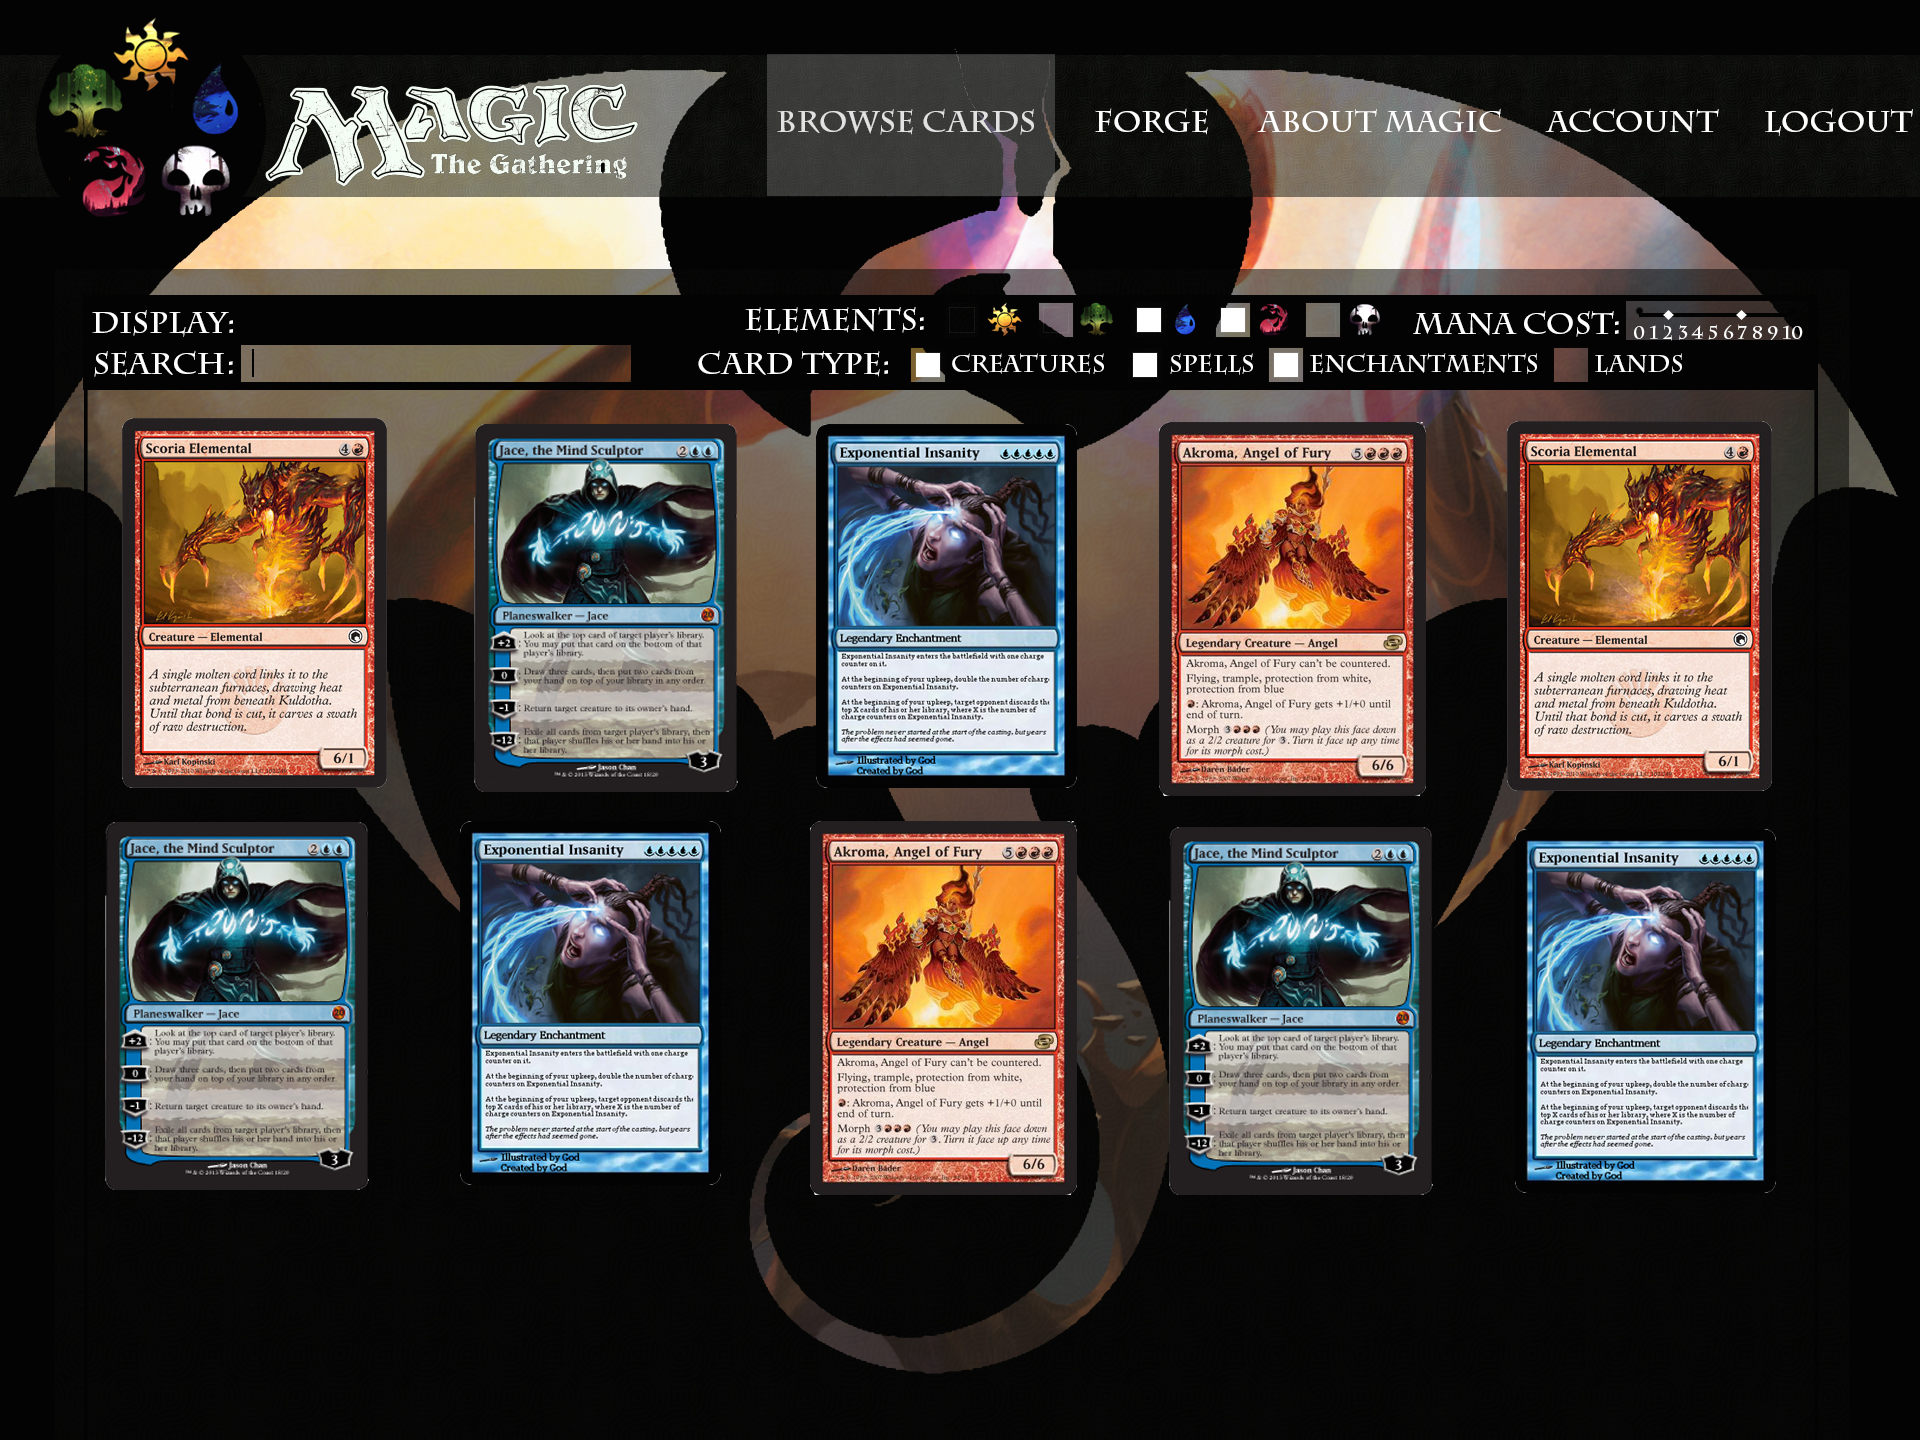
\includegraphics[width=0.8\textwidth]{FrontPage.png}}
\end{center}

\section{Navigation Diagram}
This diagram is meant as an overview of the navigation throughout the system. The diagram describes how the user navigates between pages and the two frames shows the difference in navigation when the user is logged in and when he is not.
\begin{center}
  \makebox[\textwidth]{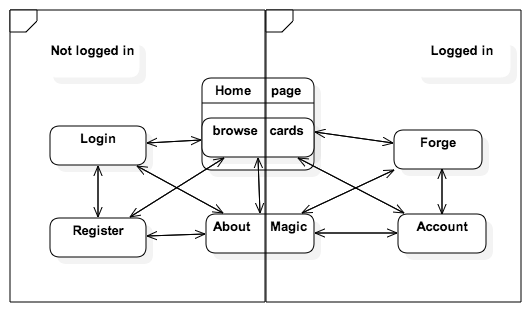
\includegraphics[width=0.5\textwidth]{StatechartDiagram1.png}}
\end{center}

\section{The Database}
Magic builder uses two different databases. All card data is pulled from an online database \href{http://api.mtgdb.info/}{http://api.mtgdb.info/} that serves json data through http GET requests. The database is accessed through a C\# driver that gives access to a library of methods that can be used to query the server for data. User data is stored in a SQL database kept locally on the server.

\section{Description of Technical Environment}
During the programming phase I will explore different ways of developing the system. The following tools have been and will be used during preparation and production of the system.
\begin{itemize}
  \item All the code behind the system will be written in Visual Studio 2013 in the MVC5 environment.
  \item For assistance I will use Sublime Text 2 while coding.
  \item The system will be designed primarily with Google Chrome making use of the built in development tools.
  \item For javascript debugging I will use jslint.com as well as the development tools in Google Chrome.
  \item Source control will be provided with git.
  \item For source control hosting, I will use github.com, and connect to github through the team explorer in Visual Studio.
  \item I will use bootstrap to make visualisation changes to the website, but also to ensure accessibility and responsiveness of the website.
  \item The prototypes are implemented in Google Spreadsheet and Photoshop.
  \item The navigation diagram was made in StarUML.
  \item Google Docs and \LaTeX \enspace was used to make the reports.
\end{itemize}

\section{Programming Rules}
I decided to put forth a few programming rules to follow, for better consistency and readability of code. First I looked at the XHTML standard for HTML and some CSS coding standards. I looked into Microsoft traditions for C\# and explored common traditions for JavaScript code. I adjusted the rules for my purposes and they are listed below with a few examples for clarity.
  \subsection{\textsc{html}}
  \begin{itemize}
    \item All attributes, events, and tags must be written in lower case.
    \item All elements must be closed.
    \item The value assigned to an attribute must be enclosed in quotes.
    \item All elements must be properly nested.
    \item Attribute minimization is not allowed (selected must be selected=`selected').
    \item Comment the code.
    \item Declare the correct doctype.
    \item Never use inline styles.
    \item Place external CSS files within the head \& put  javascript files at the bottom.
    \item Never use inline javascript.
    \item Use h1 - h6 tags properly.
    \item Use labels for all form boxes.
    \item Use unordered list for navigation.
    \item Always place the alt attribute for images.
  \end{itemize}
 \clearpage
  
  \lstinputlisting[language=HTML]{ProgrammingRules/HTMLrules.html}

  \subsection{CSS}
  \begin{itemize}
    \item When grouping selectors, keep individual selectors to a single line.
    \item Use classes in selectors but avoid id's for better reusability of code.
    \item Include one space before the opening brace of declaration blocks for legibility.
    \item Place closing braces of declaration blocks on a new line.
    \item Selectors names should start with a lowercase letter.
    \item Id names should have underscores: \#user\_image.
    \item Class names should have hyphens: .profile-image.
    \item Only use English words.
    \item Group related items together with comments.
    \item Class and id names should be descriptive.
    \item CSS files should be organized using flags.
    \item Avoid shorthand CSS.
    \item All CSS should be in an external stylesheet, no inline styles.
    \item HTML first then CSS.
    \item Comment the CSS code.
    \item Use bootstrap whenever possible.
    \item Avoid extra selectors.
  \end{itemize}
  \lstinputlisting{ProgrammingRules/CSSrules.css}
  \subsection{C\#}
  \begin{itemize}
    \item Only use English words.
    \item When code is being indented, the `tab' button should be used (in Visual Studio 2013 `tab' is saved as four spaces).
    \item Use predefined type names instead of system type names like Int32, String, Single, UInt64, etc.
    \item Use camelCasing for method arguments and local variables.
    \item Use PascalCasing for class names and method names.
    \item Use noun or noun phrases to name a class.
    \item Vertically align curly brackets.
    \item Declare all member variables at the top of a class, with static variables at the very top.
    \item Commenting Conventions:
    \begin{itemize}
    \item Place the comment on a separate line, not at the end of a line of code.
    \item Begin comment text with an uppercase letter.
    \item End comment text with a period.
    \item Should be written in English.
    \end{itemize}
    \item Always specify [HttpPost] or [HttpGet].
    \item Use a try-catch statement for most exception handling.
    \item Avoid using abbreviations in names.
    \item Do not use underscores in identifiers.
    \item Singular names for enums.
    \item Do not use the word enum in enum names.
    \item Do not push code that doesn’t compile!
    \item Avoid complex expressions.
    \item Consider warnings as errors.
    \item Set a region around code that is related to one another.
    \item Use implicitly typed local variables when the variable type is clear.
    \item Use explicitly typed local variables when the variable type is not clear.
  \end{itemize}
  \lstinputlisting{ProgrammingRules/csrules.cs}
  \subsection{JavaScript}
  \begin{itemize}
    \item In general, use camelCasing for functions, variables and methods. Use PascalCasing for classes and enums. Constant values should be in all caps.
    \item Always use semicolons.
    \item Always use ‘var’ while declaring variables.
    \item Vertically align curly brackets.
    \item Declare variables outside of the ‘for’ statement.
    \item Never pass a string to SetInterval and SetTimeOut. Instead, pass a function name.
    \item Javascript files should be stored in an external file (not inline).
    \item The code should be correctly indented.
    \item Line length should not exceed 80 characters.
    \item Variables should be declared before they are used.
    \item Use === and !== in comparisons instead of == and !=.
    \item Comment your code.
    \end{itemize}
  \lstinputlisting{ProgrammingRules/javascriptrules.js}

\clearpage

\section{The Production Process}
During the production process I worked with many tools for “bootstrapping” or creating new web apps that come prepackaged with everything a particular framework needs. While working with Angular I mostly used the \href{http://yeoman.io}{http://yeoman.io} generator which can bootstrap an Angular project with build tools included such as automated tests, package manager, source control and automated \\ deployment. After getting all of that working and setting up a webapp with some basic functionality such as a card search and some css styling I set off to get the database working, with user and card relations as well as authentication. That is where I had the most problems, getting the database to store card data and connecting that to users didn’t work. After some time I decided to move over to ASP.NET MVC5 and started from scratch there.
  
When I started on ASP.NET I decided to use the code first approach when building databases. I built some model classes for card and deck data and used code-first migrations to generate the database schema straight from the code. After dropping the database and redesigning the model classes a few times I had a working model of my data and a database to connect to. With the database layer ready I created a Repository which contains all the methods which manipulate the database, that way the database layer is completely separated from the logic and the views. By using a clear separation of the three layers replacing a layer becomes easy. After that I needed a way to pass more than one model into my views, such as Magic cards, decks and user data. I created a viewModel class that contains all the data my views need. With that taken care of I created controller endpoints for urls such as /createDeck, /search etc. with corresponding views. For easier styling I added bootstrapLess which is an extended .less version of the popular Bootstrap UI css style framework.  Less allows the designer to think more like a programmer while adding styling to pages. Less uses functions, variables and selector nesting for easier development. When the project is built the .less files are converted to .css. Finally, after the core functionality regarding search and decks was completed I added a details pop up view for individual cards and did some refactoring on the code, such as putting repeated html into partial views to reduce clutter in the Razor view pages. I added filters to the search to be able to narrow down card choices and then I deployed the app to a cloud based server hosted with Microsoft.
\subsection{How the overall production fared}
I initially started building the system using AngularJS along with an online database \href{http://www.firebase.com}{www.firebase.com}. I had some trouble getting things to work, especially concerning the database connections. In the end I decided that AngularJS framework was too large and complex for the simple functionality of Magic Builder so I abandoned that approach in favor of using asp.net MVC5. Having had no experience with neither of those systems I spent a lot of time doing tutorials and reading about how things work. I also started from scratch a few times in order to eliminate design errors while building the database and models. Getting the initial system to build, connecting the database and enabling user accounts was challenging but after a view tries I got things working. 

\clearpage

\subsection{What went wrong and how it can be done better next time
}
While working on the project I spent a lot of time on setting up new Angular and ASP.NET MVC5 web apps, configuring databases and managing authentication. On my next project I know I will be much better familiarized with the frameworks which will cause me to design the inner workings of the system in accordance with the frameworks. I can than hopefully avoid design errors which led to me starting from scratch a few times.
At the start of the project while I worked with AngularJS I had some problems setting up a database connections with \href{http://www.firebase.com}{www.firebase.com}, in the future I will be wary of using bleeding edge technologies such as the Angular and Firebase wrapper AngularFire, lack of examples and documentation proved problematic.
After I connected to the online Magic the gathering database with the MtgDb.driver.dll available on \href{http://api.mtgdb.info/}{http://api.mtgdb.info/} I noticed that I was getting parse errors on some JSON data so that the search feature was completely broken, fortunately someone had posted details about the error on the projects \href{https://github.com/planeswalkers/CSharpMtgDb.Info}{github site}. After cloning the project i was able to locate the problematic code, fix it and rebuild the .dll file. Everything worked like a charm after that.

\section{Requirements Outcome}
\begin{center}
  \makebox[\textwidth]{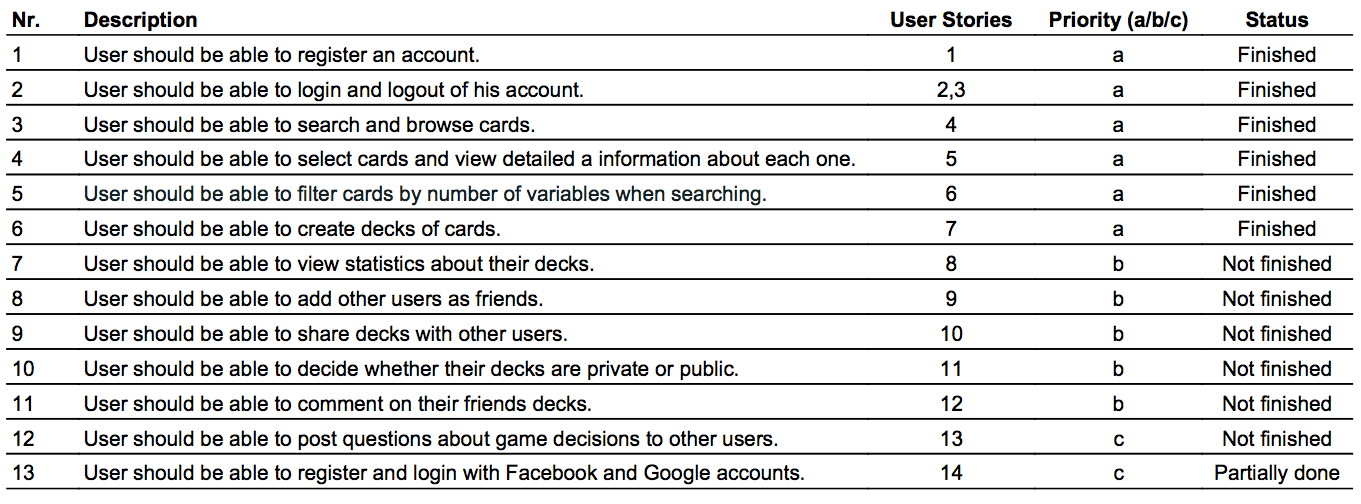
\includegraphics[width=1\textwidth]{RequirementsRevised.png}}
\end{center}
\begin{center}
  \makebox[\textwidth]{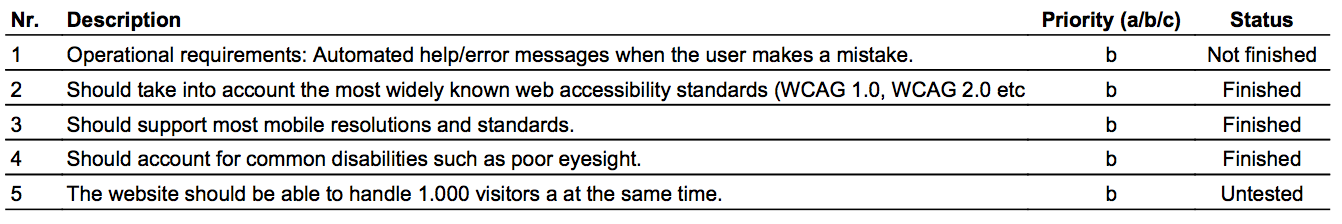
\includegraphics[width=1\textwidth]{NonFunctionalRequirementsRevised.png}}
\end{center}
\clearpage
\subsection{What Requirements were met}
The main goal of this project was to finish the fundamental requirements and during the implementation learn more about the overall setup of a web application. The initial step was to allow users to register an account, login and log out. The MVC ASP.NET framework in Visual Studio offers a premade authentication which I could use as a base for MagicBuilder. The built in functionality for the project did help in some areas but not in all. Nevertheless, I decided to try to use as much of it as I could since it offers a lot of perks, such as input validation and security for database records. The account requirements were therefore quite straightforward to implement although I needed some research to make my own tables connect with the user table as to make sure that each user had separate decks and saved cards.
  
The second part of the project became the search. I started by making a simple search where the user could input a search input string and get all cards that contained that particular string in their name. The user is presented with no more than 100 cards that he can browse through. When I got further into the project and got more comfortable with the online database I added a few filters to the search. The filters allow the user to narrow down their search a bit which is much more user friendly. I found it unnecessary to add more filters since the project is only meant as a prototype.

Each card presented by the search also includes a detailed information about itself. Since the cards themselves are sometimes hard to read I felt it was important that the user could view these details in a larger window. I added a flip over effect on the cards that presents a button that the user can press for more details about the card. It provides a nice visual as well as a simple interface for the user. When the user presses the button a window is displayed while the surroundings are blurred so the window becomes very clear and the user is not interrupted by other material. The window displays the card image a bit larger and all relevant data related to that card.

The main reason for making an account based application was to allow the user to create his personal decks and add cards to them. It took a bit of time to get my database tables to work with the user database as well as the online database but when the connection had been properly made I made a tab bar where the user can create and view his decks. I also created a rename and delete deck functions which I felt was important for the usability of the system. The ‘add to deck’ and ‘remove from deck’ buttons were placed on the backside of the cards with the ‘detail’ button for good consistency.

The non-functional requirements were not a high priority. Nevertheless, I tried to keep them in mind as I worked and managed to finish a few of them.

Overall I am very pleased with the progress of the high priority requirements. I feel that the system now offers a good base for a larger project and it should be great foundation to built upon.

\subsection{What Requirements where not finished and why}
Since this project was meant as a study of basic web development, I decided to focus on finishing the highest priority requirements and try to implement them so as to make the system a good mini version of a system of this type. All lower priority requirements were therefore left out, i.e. all B and C requirements, since all extra time was spent on optimizing the high priority requirements rather than adding more features.

All non-functional requirements were B or moderate priority. Even so, some of them I managed to finish but the help and error messages are not finished. There is some input validation and there aren't many places where the user can make mistakes so these messages should be one of my future goals.

\section{Usability Goals Outcome}
The usability goals were put forth to make sure that the features implemented were simple and easy to use. No formal usability test was conducted, although I did test the system informally on another user that had no trouble finishing the task required in the time limit given by the usability goals. I felt it was very helpful to have formulated these goals since it made me think more on how the user would actually use the system and not only on how it would work. I believe that during web development it is especially important to not forget the user and always try to envision the user’s responses to the interface and its functionality.

\section{Changes from Initial Analysis and Design}
\subsection{Interface Design}
My main frame of reference for the interface design were the wireframes. I made the graphic design models more as inspiration but I always suspected that the project’s timeframe would not allow for such an extreme design. I also felt it was more important that the website was responsive so I decided to use bootstrap as much as possible. The layout of the page turned out quite similar to the wireframes, although, in the forge where the user can make decks and search for cards, I decided to have the decks content listed above the search and not the otherway around like in the wireframes. Furthermore, some of the top nav bar links have other names than I originally planned, but still the layout is quite similar.
\subsection{The Navigation Diagram}
Although the navigation diagram was very simple I feel it helped me visualize the overall navigation throughout the website. I decided to keep the navigation as I originally designed although some names changed and I left out the ‘about Magic’ site since it didn’t require any programming and was therefore a bit unnecessary for this project.

\section{What was Learned}
This project increased my understanding of web development considerably. I feel that I have a much better grasp of the MVC concept and how the three layered design works when working with web applications.
  
Researching, doing tutorials and building the AngularJS project gave me a lot of experience coding in Javascript , working with Javascript frameworks and manipulating data in the JSON format.

Web programming in ASP.NET was completely new to me so I spent some time reading about how it works and after that came countless tutorials and finally the project itself. I now have a good understanding of how the ASP.NET MVC5 model works, how to code the controllers, work with Razor views to bind data into views and compile HTML, manipulate the configuration files, manage databases, work with source control in Visual studio and deploying the webapp to a live server.

\clearpage

\section{Conclusion}
Overall I am very happy with how the project turned out, I accomplished my goals regarding learning the technologies needed to become a more valuable member at work.
The webapp is simple and there are still a lot of features I’d like to add, such as layout and style changes, error handling, deck information and probability statistics but the system works and is now running on a live server at \href{http://magicbuilder.azurewebsites.net/}{http://magicbuilder.azurewebsites.net/}. 
\\ The code is available at \href{https://github.com/svavarhall/MagicBuilder}{https://github.com/svavarhall/MagicBuilder}. I fell like I'm just getting started with the system so I will undoubtedly continue development over the summer and hopefully I can get it to a stage where me and my friends at work can start using it to track scores, look at statistics and other related things during our weekly Magic sessions. 

\clearpage

\section{References}

\href{http://en.wikipedia.org/wiki/Magic:_The_Gathering}{Further information about Magic the Gathering, the card game.}
\\ \href{http://www.mtgvault.com/}{mtg vault}
\\ \href{http://api.mtgdb.info/}{http://api.mtgdb.info/}
\\ \href{http://yeoman.io}{http://yeoman.io}
\\ \href{http://www.firebase.com}{www.firebase.com}
\\ \href{https://github.com/planeswalkers/CSharpMtgDb.Info}{The Github site for the Magic Database}
\\ \href{https://docs.angularjs.org}{The official AngularJs documentation}
\\ \href{https://egghead.io/}{Egghead.io - a source of AngularJS tutorials}
\\ \href{https://thinkster.io/}{Thinkster.io - a source of AngularJS tutorials}
\\ \href{http://www.asp.net/mvc}{asp.NET MVC official tutorials portal}
\\ \href{https://azure.microsoft.com/en-us/documentation/}{Microsoft azure web services documentation}

\end{document}
